\chapter{OPTIMAL INTERPOLATION TO IMPROVE SATELLITE NOWCASTS WITH DATA}
\label{chap:satoi}

references to other sections
- application
- basic background
- results

\section{Satellite to Irradiance Algorithms}
- high res requirements
- GOES, time res
- why geostationary

\subsection{UASIBS Model}
The University of Arizona Solar Irradiance Based on Satellite (UASIBS)
model was developed at by Chang Ki Kim in 2015 \citep{Kim2016}.
This model relies on the infrared images of the GOES-W satellite to
find completely overcast areas based on a comparison of the brightness
temperature difference (difference between 10.7 and 3.9 $\mu$m
images) to a reference calculated over the past few weeks.
If the infrared channels do not find an area to be overcast, the
visible image is compared to a threshold image to determine if any of
the 16 pixels in the 4km $\times$ 4km box have a cloud.
Once pixels are classified as cloudy or clear, a look-up table is
employed to find the atmospheric transmittance and GHI on the ground
for each pixel.
A number of look-up tables are generated from using Goddard Space
Flight Center Radiative Transfer Model: one for clear sky
accounting for aerosols, one for high level clouds, one for mid level
clouds, one for low clouds, and one for cumulus clouds.

The look-up table approach to calculate transmittance is limited.
First, a number of climatological averages, specific to Tucson, are
used in the calculations of the look-up tables including AOD and
ozone.
Instead, near real-time analysis and forecasts of AOD and ozone are
available from Monitoring atmospheric composition and climate (MACC)
project \citep{Morcrette2009} and a ground truth measurement of AOD is
available from the Tucson AERONET site \citep{Holben1998}.
Another limitation is that only ten values of the solar zenith angle
are used which introduces artificial steps noticable in the output
GHI.
With newer, fast radiative transfer codes, perhaps the look-up table
approach can be replaced with a direct call to a radiative transfer
code to avoid this issue.

\begin{figure}[h]
\centering
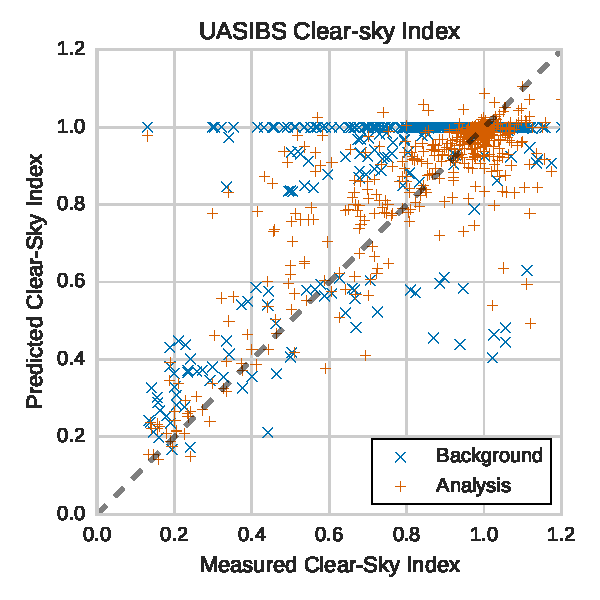
\includegraphics[width=0.7\textwidth]{figs/uasibs_scatter.pdf}
\caption[Scatterplot of predicted vs measured clear-sky index for
UASIBS]{A scatterplot of the predicted vs measured clear-sky index for
UASIBS before OI (blue) and after (orange). It is obvious there is
some issue where UASIBS does not produce clear-sky indices between 0.6
and 0.8. OI helps correct this somewhat. (Reproduced from
\cite{Lorenzo2017})}
\label{fig:uasibs_scatter}
\end{figure}

The cloud detection methodology may also have issues when classfying
clouds to use one of the look-up tables.
This is illustrated in Fig.\@ 4 of \cref{app:satoi} reproduced in
\cref{fig:uasibs_scatter}.
There is a distinct lack of images with clear-sky index between 0.6
and 0.8 for UASIBS (blue $\times$s) that requires further
investigation to determine if it is a problem with the look-up tables
themselves or using the wrong look-up table.
Removing the classification of cloud type and calculating the
radiative transfer directly will likely solve this issue.

\subsection{Semi-Empirical Model}
The semi-empirical model used and described in \cref{app:satoi} is
based on what is commonly know as the SUNY model developed by Perez
\etal \citep{Perez2002}.
This model was chosen because it is well known within the community
and provides a good benchmark.
The SUNY model was developed using ground truth sensors spread
throught the US with few in arid climates and no sensor in Arizona.
Notably, Perez \etal recognized the deficiency in arid areas with high
ground albedos and proposed a method to correct this issue
\citep{Perez2004}.
The high ground albedo combined with the empirical coefficients
developed for the US broadly likely lead to the overprediction of
cloudy skies in \cref{fig:suny_scatter}.

\begin{figure}[h]
\centering
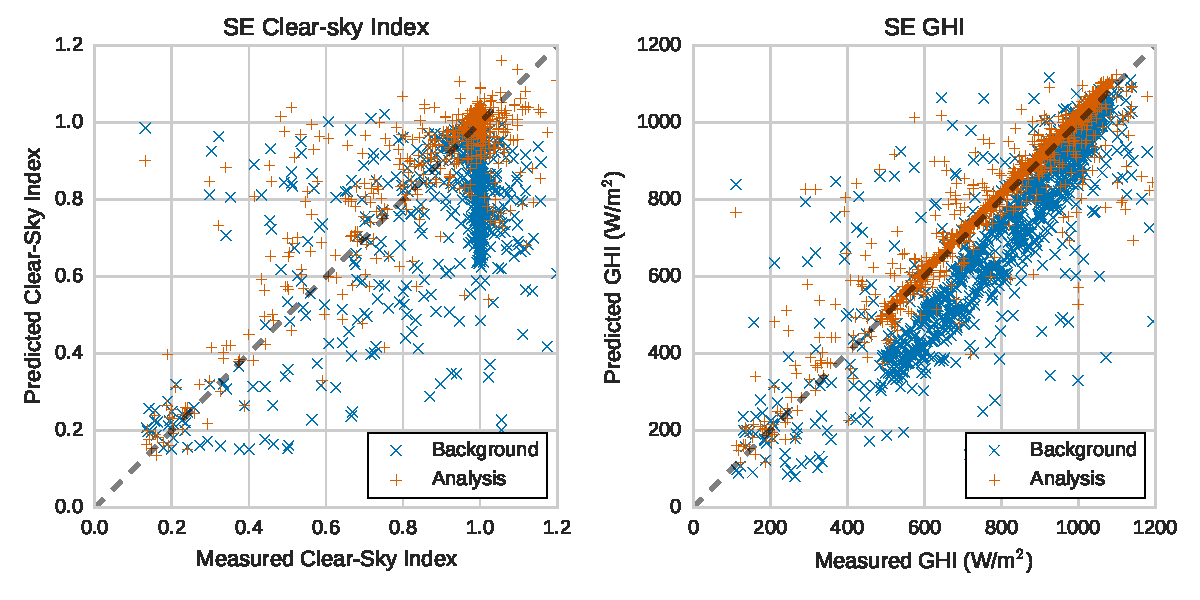
\includegraphics[width=\textwidth]{figs/suny_scatter.pdf}
\caption[Scatterplot of predicted vs measured clear-sky index for the
semi-empirical model]{A scatterplot of the predicted vs measured
  clear-sky index for semi-empirical model before OI (blue) and after
  (orange). The semi-empirical model tends to overpredict clouds as
  shown in the clear-sky index scatterplot on the left. The splitting
  for the GHI in the right image is likely due to a time of day
  effect.  (Reproduced from \cite{Lorenzo2017})}
\label{fig:suny_scatter}
\end{figure}

A new, more strict test of OI in southern Arizona would be to
recalculate the empirical coefficients used in the semi-empirical
model for the area.
This would likely improve the background errors of the semi-empirical
errors and may also improve the final errors after performing OI.

\subsection{Other Models}
There are numerous algorithms to convert satellite measured radiances
to ground irradiance.
A good overview of semi-empirical and physical methods can be found in
\cite{Perez2013a,Miller2013}.

One publicly available dataset is the GOES Surface and Insolation
Products (GSIP).
GSIP provides hourly irradiance estimates at a resolution of 1/8
degree.
OI is unlikely to perform well with this low spatial resolution
({\raise.4ex \hbox{\texttildelow}}14km) where clouds are not well
resolved and many sensors are contained in a single grid cell.

The National Renewable Energy Laboratory (NREL) is developing a new
algorithm called the Physical Solar Model (PSM) that has been used to update
the National Solar Radiation Database (NSRDB).
NSRDB provides 30 minute 4km $\times$ 4km data covering the US (and
some other countries) from 1998 to 2015.
One could explore how OI performs for an NSRDB background, but the low
spatial resolution may prove limiting.
Furthermore, the PSM algorithm is currently unpublished so it cannot
be used to make operational nowcasts which is the ultimate goal of OI.

\subsection{Future Models}
With the launch of GOES-16 a number of groups are developing products
and algorithms that make use of the new Advanced Baseline Imager
(ABI).
The new ABI will image the continental US every five minutes with 16
spectral bands and resolutions as high as 0.5 km for the 0.64 $\mu$m
visible band.
Pictures of a comparison of the new GOES-16 and the current GOES-13
visible images in \cref{fig:goes_comp} and of a detailed image over
California in \cref{fig:goes_cal} show the impressive capabilities of
the instrument.

\begin{figure}[h]
\centering
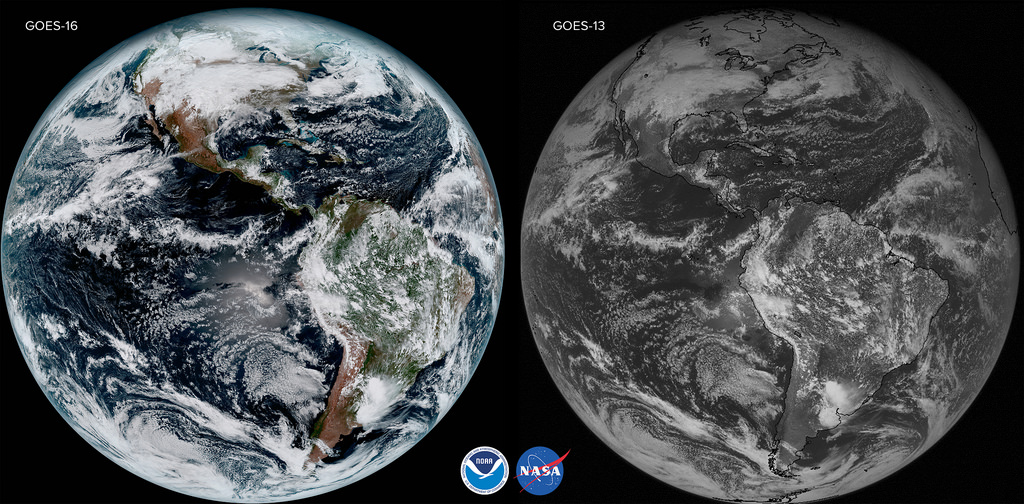
\includegraphics[width=\textwidth]{figs/goes_comp.jpg}
\caption[Comparison of visible images from the current and future
GOES]{A comparison of visible images created from the visible channels
of the new GOES-16 satellite and the previous generation
GOES-13. GOES-13 has only a single visible channel while GOES-16 has
three. Image courtesy of NOAA.}
\label{fig:goes_comp}
\end{figure}

\begin{figure}[h]
\centering
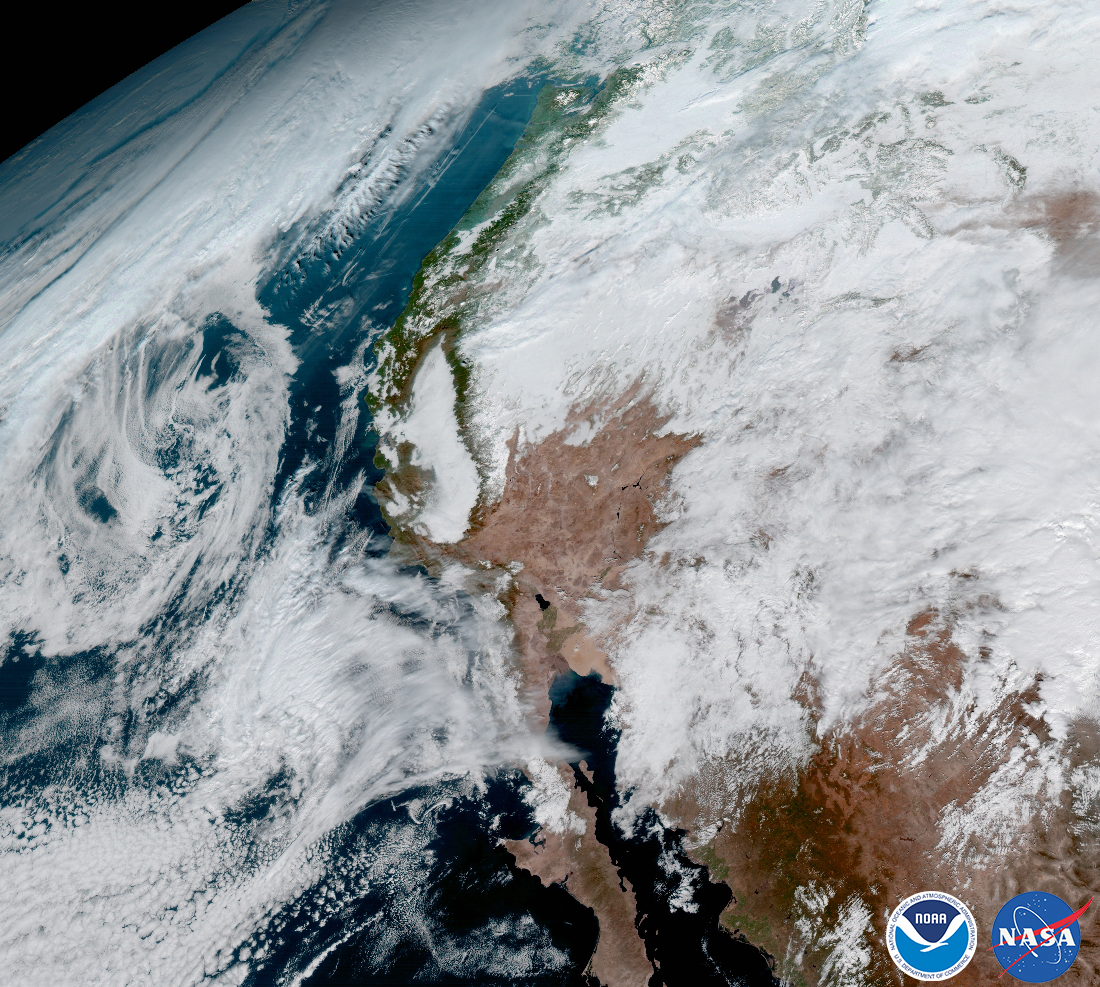
\includegraphics[width=0.7\textwidth]{figs/goes_cal.jpg}
\caption[An visible image of the western US from GOES-16]{A visible
image of the western US from the new GOES-16 satellite. The improved
resolution and spectral bands will improve satellite derived
irradiance estimates compared to the current generation of
satellite. Image courtesy of NOAA.}
\label{fig:goes_cal}
\end{figure}

This higher spatial resolution will make it all the more important
to minimize cloud location errors with respect to the ground sensors.
It is possible that OI will show little gain over GHI estimates using
these new ABI capabilities.

\section{Parameter Estimation}
\label{sec:paramopt}

Section 6 of \cref{app:satoi} discusses the tuning of OI for a
specific location including the estimation of the parameters $k,\:
l,\: d$ by minimizing the mean-squared error (MSE) of the analysis
over sensors withheld from OI.
To perform this minimization a grid search over the parameters was
performed and the resulting MSE for each set of parameters is shown in
\cref{fig:paramopt}.
This figure clearly shows distinct minima in parameter space for the
UASIBS satllite to irradiance model which indicates that  OI is
sensitive to the choice of parameters.
On the other hand, the lack of distinct minima in parameter space for
the semi-empirical model indicates that a wide range of parameters would
give similar results after performing OI.
If in the future the semi-empirical model is chosen as the background model
for an OI based routine, a more thorough investigation into why OI is
insensitive to these parameters is warranted.

\begin{figure}[p]
\centering
\captionsetup[subfigure]{labelformat=empty}
\subfloat{\hspace{-1em} 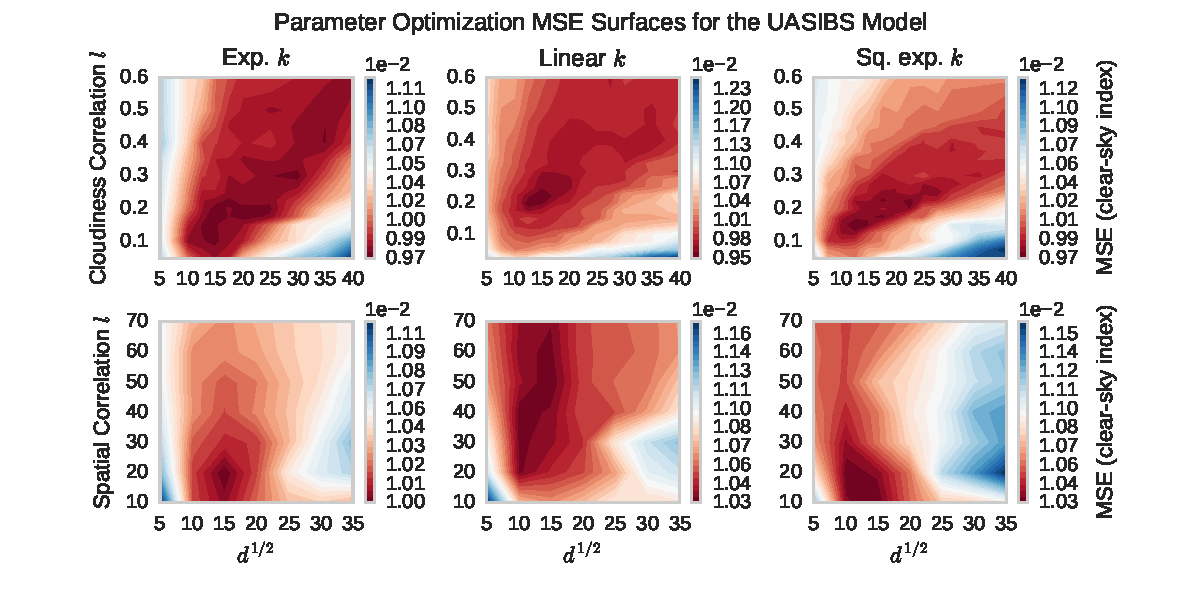
\includegraphics[width=1.05\textwidth]{figs/uasibs_optsurf.pdf}}
\vspace{-1em} \\
\subfloat{\hspace{-1em} 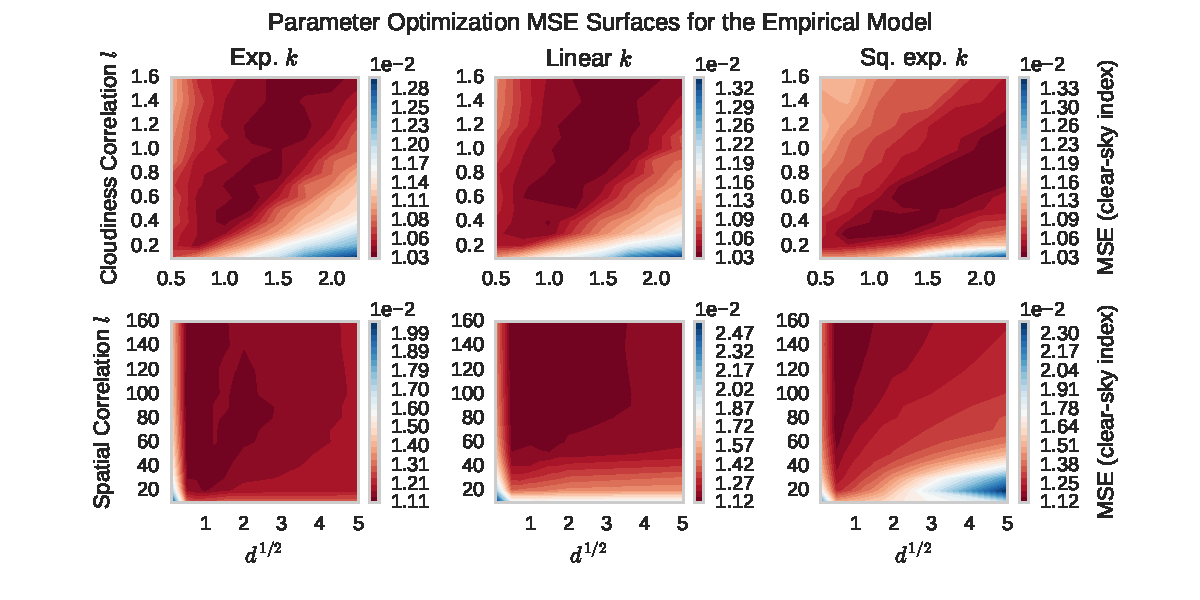
\includegraphics[width=1.05\textwidth]{figs/suny_optsurf.pdf}}
\caption[Optimization surfaces for OI parameters]{Optimization
  surfaces for the parameters $k,\: l,\: d$ of the optimal
  interpolation routine. The columns represent different choices of
  $k$, the rows distinguish between cloudiness and spatial
  correlation, the y-axis is $l$ and the x-axis is $d^{1/2}$. The top
  figure shows surfaces for the UASIBS model and the bottom is for the
  semi-empirical model. Note, that for all choices of $k$ and the
  correlation parameterization, the surfaces for the UASIBS model have
  a clear minimum. The surfaces for the semi-empirical model have less
  distinct minima indicating that optimal interpolation is not
  particularly sensitive to parameter choice for this model.}
\label{fig:paramopt}
\end{figure}

\section{Future Work}
(mainly pertaining to OI, mabye little bit of kalman)

layers

new sat to irr algorithm

Here is some future work

%%% Local Variables:
%%% mode: latex
%%% TeX-master: "dissertation"
%%% End:
